\documentclass[12pt,a4paper]{article}
\usepackage[
	left 	= 2.5cm,
	right 	= 2.5cm, 
	top 		= 2.5cm,
	bottom 	= 2.5cm,
]{geometry}
\usepackage[utf8]{inputenc}
\usepackage[english]{babel}
\usepackage[OT1]{fontenc}
\usepackage{amsmath}
\usepackage{mathtools}
\usepackage{graphicx}
\usepackage{caption}
%\usepackage[round]{natbib}
\usepackage[style=apa, backend=biber]{biblatex}
\addbibresource[]{ref.bib}

\usepackage[hidelinks]{hyperref}
\hypersetup{
	colorlinks = true,
	urlcolor   = blue,
	linkcolor  = black, 
	citecolor  = blue, 
}


\usepackage{fancyhdr}
\pagestyle{fancy}
\lhead{\slshape Unterweger}
\chead{}
\rhead{\slshape \nouppercase{\leftmark}}

\usepackage{titlesec,xcolor}
\titleformat{\section}{\bfseries}{\thesection}{0.5em}{}
\titlespacing{\section}{0pt}{3ex plus 1ex minus 0.2ex}{10pt}
\setlength{\headheight}{14.49998pt}

\usepackage{titlesec,xcolor}
\titleformat{\subsection}{\bfseries}{\thesubsection}{0.5em}{}
\titlespacing{\subsection}{0pt}{3ex plus 1ex minus 0.2ex}{10pt}
\setlength{\headheight}{14.49998pt}


%------------------------------------------------------------------%

\author{Lucas Paul Unterweger}
\title{Beyond the bin: An Analysis of Waste Generation and its Environmental Consequences}


\begin{document}

\begin{titlepage}
\center
\vfill

\includegraphics[scale=0.15]{UIUC.png}
\vfill
\begin{tabular}[t]{lc}
Course:  & ECON 450 - Environmental Economics \\
Examiner: & 
Dr. Bryan Buckley \\
Submission date: & 10th of December 2023 \\
\end{tabular}
\vfill
{\large \textbf{Beyond the Bin: An Analysis of Waste Generation and its Environmental Consequences}}
\vfill
by\\ \vspace{3mm}
{\Large Lucas Unterweger \href{https://github.com/therealLucasPaul}{
\includegraphics[scale=0.01]{GitHub.png}}}\\
(UIN. 668947972)\\
\vfill

\thispagestyle{empty}
\pagebreak
\end{titlepage}
\newcounter{savepage}
\pagenumbering{roman}
\thispagestyle{empty}
\begin{abstract}
\textit{Lorem Ipsum....} 
\end{abstract}
\clearpage
\thispagestyle{plain}
\tableofcontents
\pagebreak
\setcounter{savepage}{\arabic{page}}
\pagenumbering{arabic}
\section{Introduction}
In 2018, researchers at \textit{The Ocean Cleanup Foundation} estimated that the Great Pacific Garbage Patch consists of at least 79 000 tons of ocean plastic within an area of roughly 1.6 million square kilometres. \parencite{lebreton2018} Additionally, the UN Environment Program (UNEP) has published a report in 2021 expecting plastic pollution in the oceans to nearly triple by 2040, "adding 23-37 million metric tons of waste into the ocean per year." \cite{UN REPORT} Seeing these figures and keeping in mind that widespread and uncontrolled plastic pollution causes serious issues for humans as well as animals, it is apparent that this environmental issue is a problem policy makers yet have to find an answer for. To tackle such an issue, it often is worthwhile to take a look at the source of the problem and thus this paper will take a look a municipal waste generation of countries and its development in recent years. Before advancing it might be helpful to accurately define \textit{municipal waste}, which according to the OECD is as follows:

\begin{quote}
Municipal waste is defined as waste collected and treated by or for municipalities. It covers waste from households, including bulky waste, similar waste from commerce and trade, office buildings, institutions and small businesses, as well as yard and garden waste, street sweepings, the contents of litter containers, and market cleansing waste if managed as household waste. The definition excludes waste from municipal sewage networks and treatment, as well as waste from construction and demolition activities. This indicator is measured in thousand tonnes and in kilograms per capita. \parencite{OECDData}
\end{quote}

Similarly to a variety of environmental issues, the costs that individuals or companies have to bear often only reflect the service of transporting the generated waste to a landfill or some industrial facility that purposes or burns the waste. However, these prices often neglect the hidden price that amassed can have on nature and humans as the Great Pacific Garbage Patch shows. The city of Vienna for example offers a service which picks up garbage from buildings and charges based on the amount of pick-ups per year and the maximum weight of every pick-up. \parencite{MA48} Were these prices to accurately reflect the social costs the waste produces, it would need to depend on what type of waste was generated - plastic, paper or biological - and were it would end up at the end - a landfill, garbage incinerator or recycling center. This however would need logistical and financial resources as well as a plan to circumvent the time restrictions which a city alone could hardly allocate, thus leading to a discrepancy between social and private cost. 


\section{Data Source}
Reliable data on waste generation is often hard to find and if so, it often only captures one part of the entire picture. Various sources only include waste produced by households and thus ignores the waste produced by companies, other sources are only infrequently collected by academic parties or organisations. Two of the few reliable sources for this kind of data out there are  \textit{Eurostat} and the \textit{Organization for Economic Cooperation and Development (OECD)}. The latter regularly publishes freely accessible yearly time series data on municipal waste generation in total tonnes and in tonnes per capita for a wide range of countries. The most recent data set includes 53 countries - the majority being developed nations from Europe and South East Asia as well as the United States and Mexico - along with aggregated data on the 27 member states of the European Union and the OECD. \parencite{OECDData} Unfortunately, data points are rare for years prior to 1995 and thus regularly having data points with more than 40 countries is only from then onwards. 

\pagebreak
\section{Data Analysis}

Moving on to the descriptive data analysis which will be done using the statistical programming language R \textcite{RLanguage} along with it's open source packages. The code that has been used to create these plots can be found on GitHub via the following \href{https://github.com/therealLucasPaul/ECON415_EnvEcon}{link}. First, it might be useful to have a look at the raw data itself. Due to the long history of collecting this type of data by \textit{Eurostat}, the quality of the data is generally best for EU member states specifically but European countries in general. In figure \ref{fig:wastegen_Europe} a time series plot of the municipal waste generation for European countries in kilograms per capita between 1995 and 2021 is presented. In general, a slight upward trend can be observed. 
\begin{figure}[h]
\centering
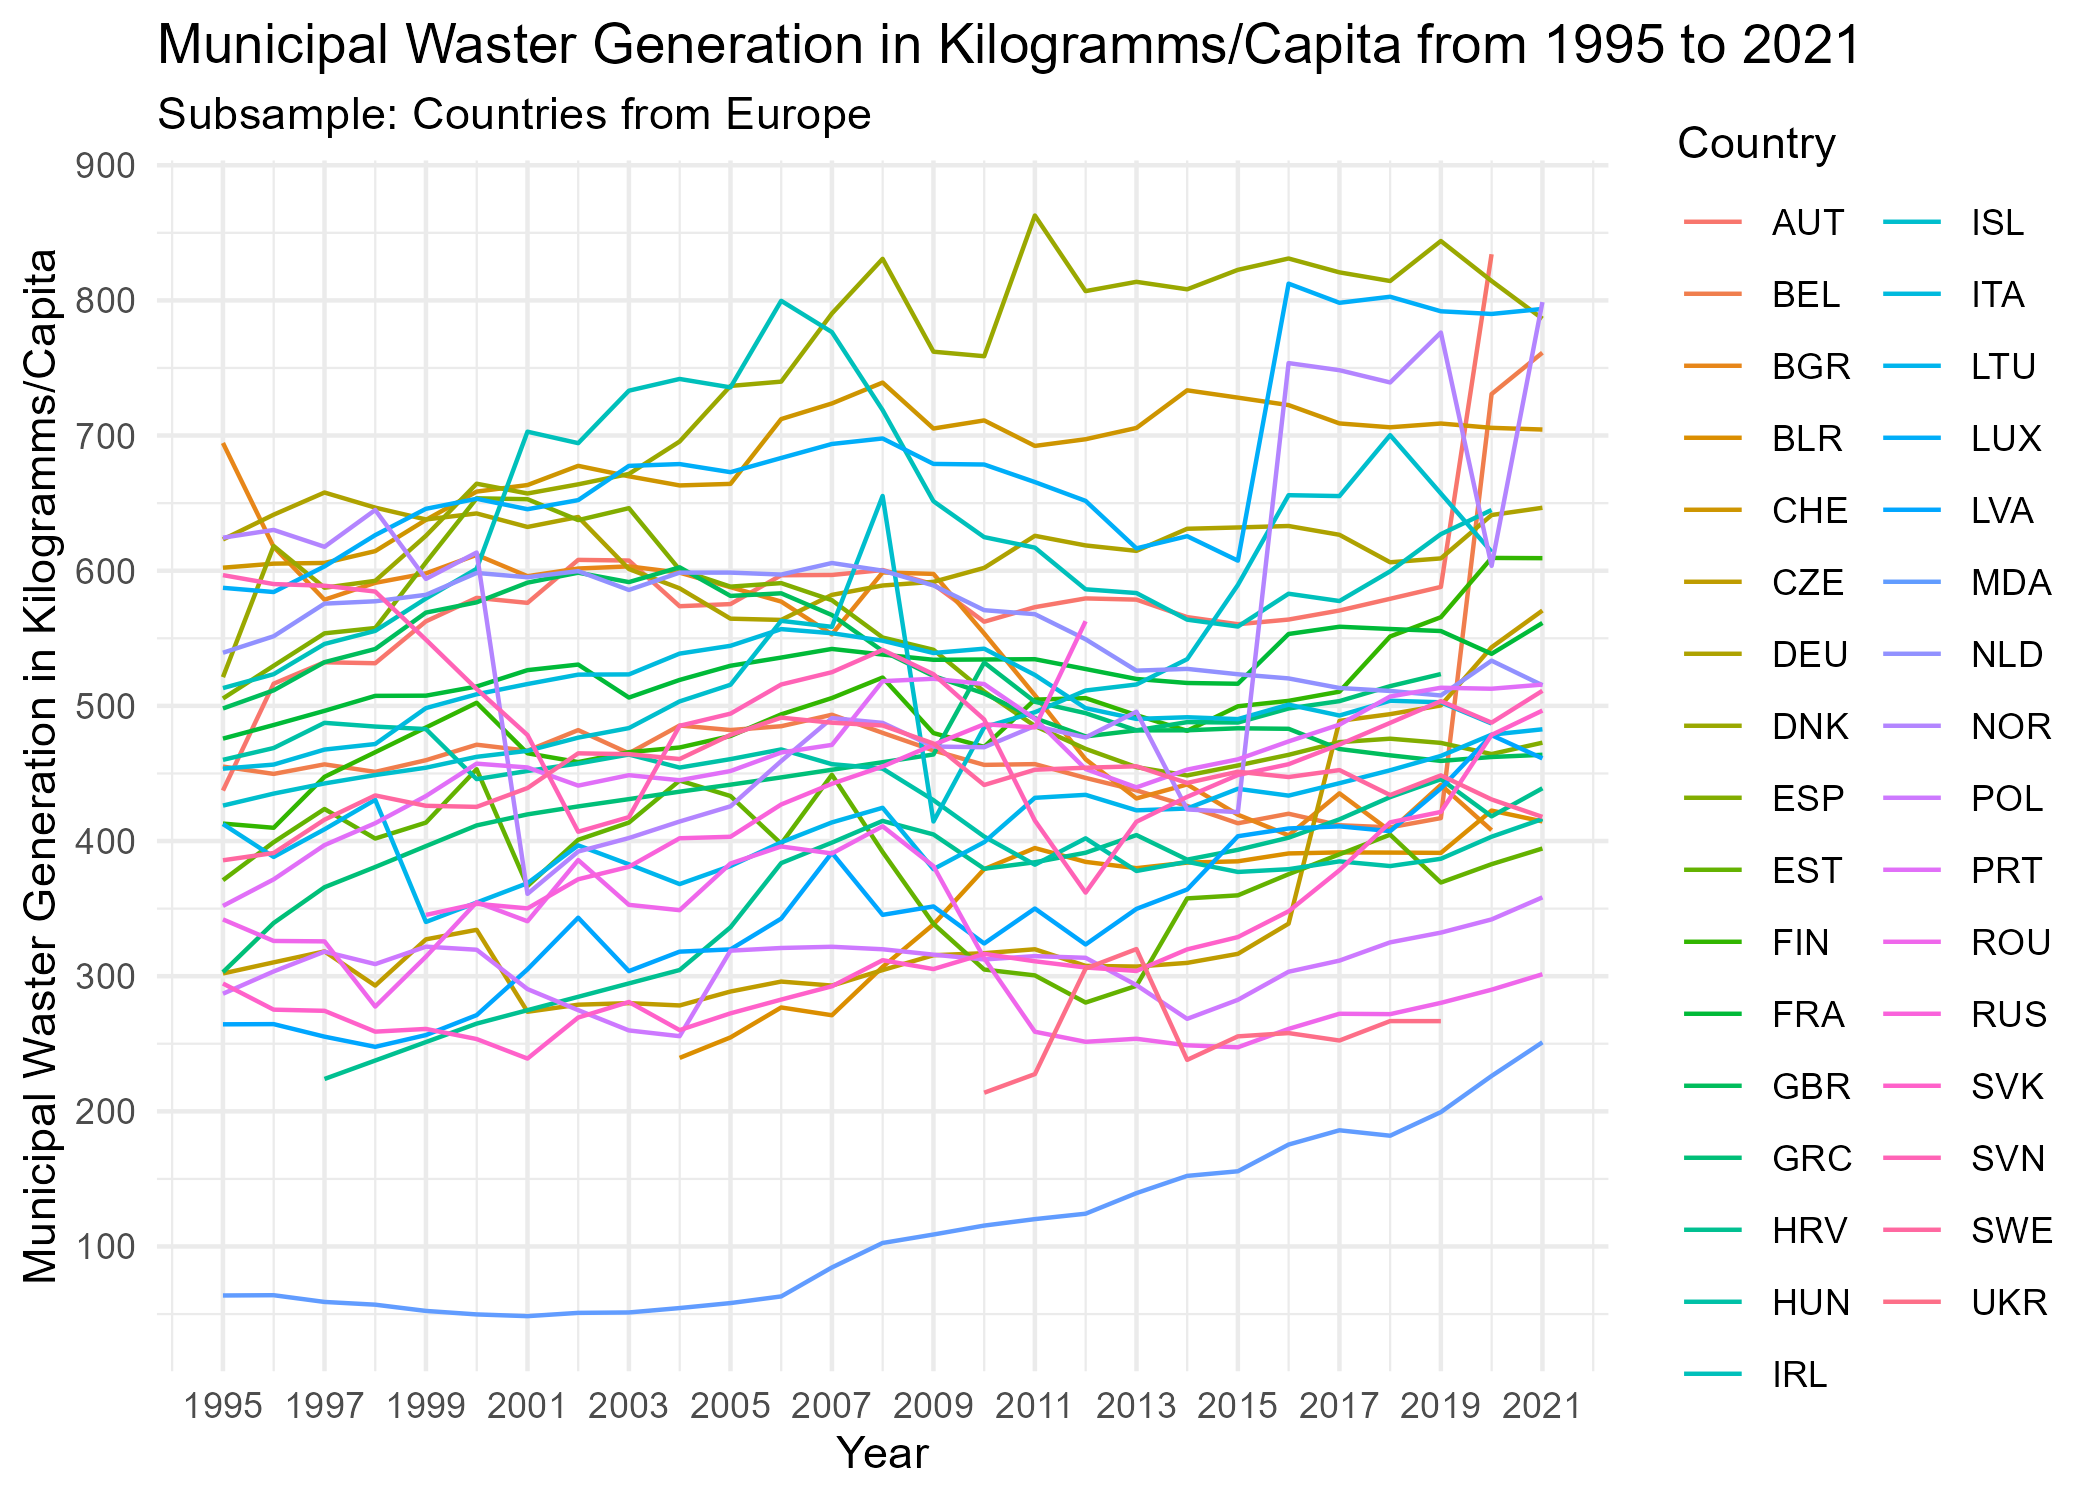
\includegraphics[scale=0.8]{../04_figures/wastegeneration_Europe.png}
\caption{Municipal Waster Generation in Kilogramms/Capita from 1995 to 2021}
\label{fig:wastegen_Europe}
\end{figure}

In general, the average year on year growth rates tend to be positive for most countries in the observed period of time as can be seen from figure \ref{fig:histgrowthrates} in the appendix, where a histogram of the rates is presented. With a mean average year-on-year per capita growth rate of $1.64\%$ and a median rate of $1.05%$, countries generally have increased their municipal waste generation in recent years. The outlier on the right represents Argentina, which is a result of the poor data availability. After closer examination it can be seen that the main driver between the smaller growth rates are non-European countries whereas the higher growth rates can mainly be contributed to European countries. 

\pagebreak
\begin{figure}[h]
\centering
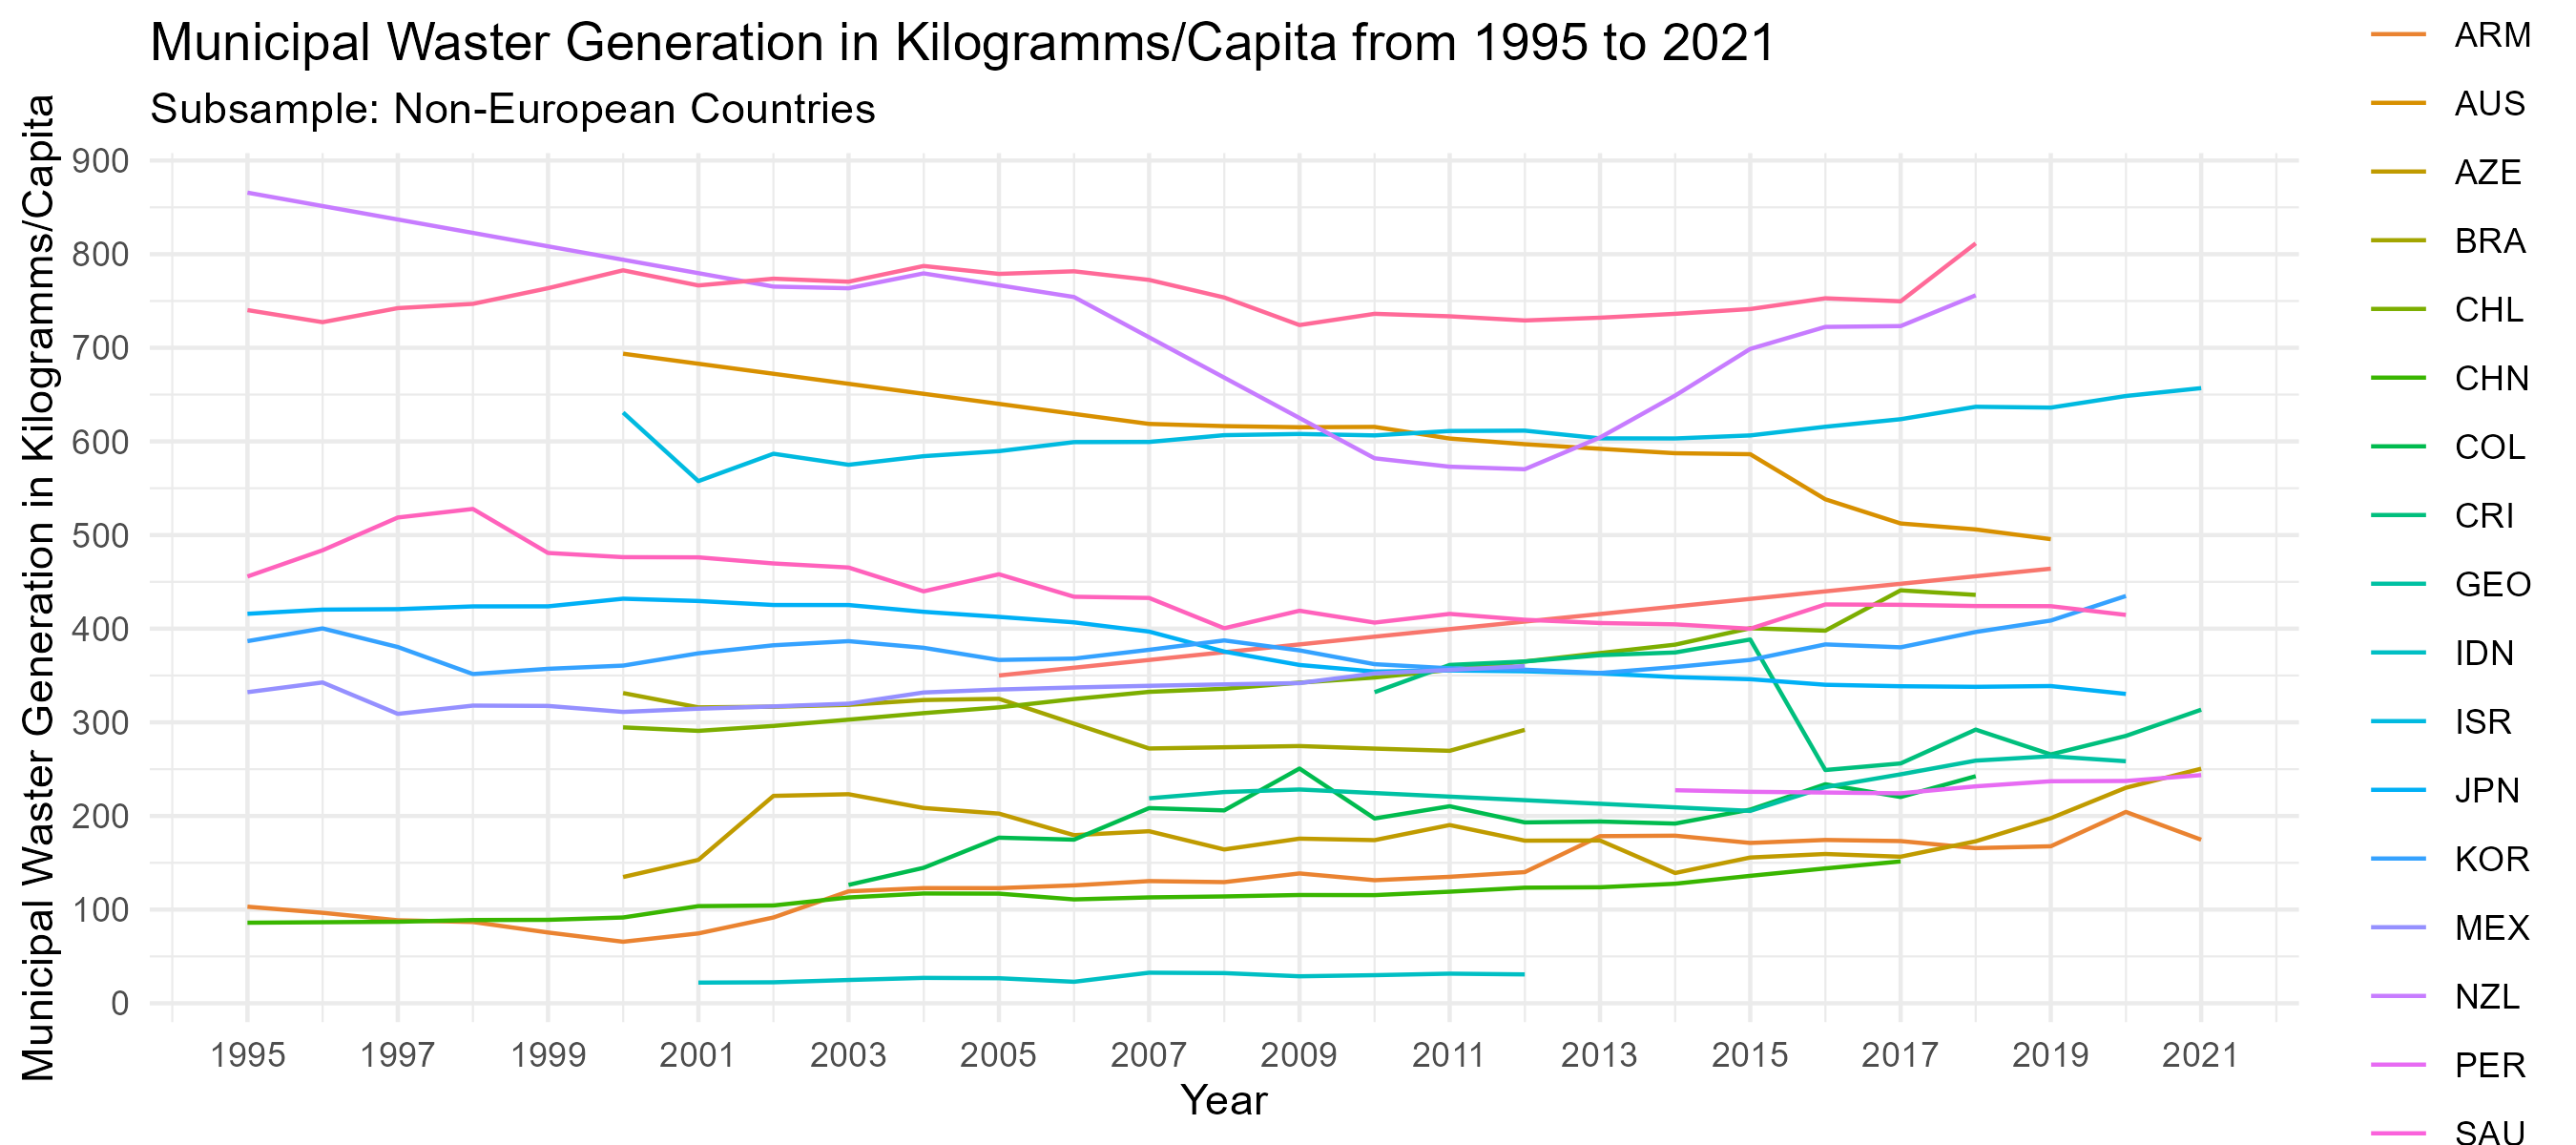
\includegraphics[scale=0.8]{../04_figures/wastegeneration_NonEurope.png}
\caption{Municipal Waster Generation in Kilogramms/Capita from 1995 to 2021}
\label{fig:wastegen_NonEurope}
\end{figure}

\pagebreak
\begin{figure}[h]
\centering
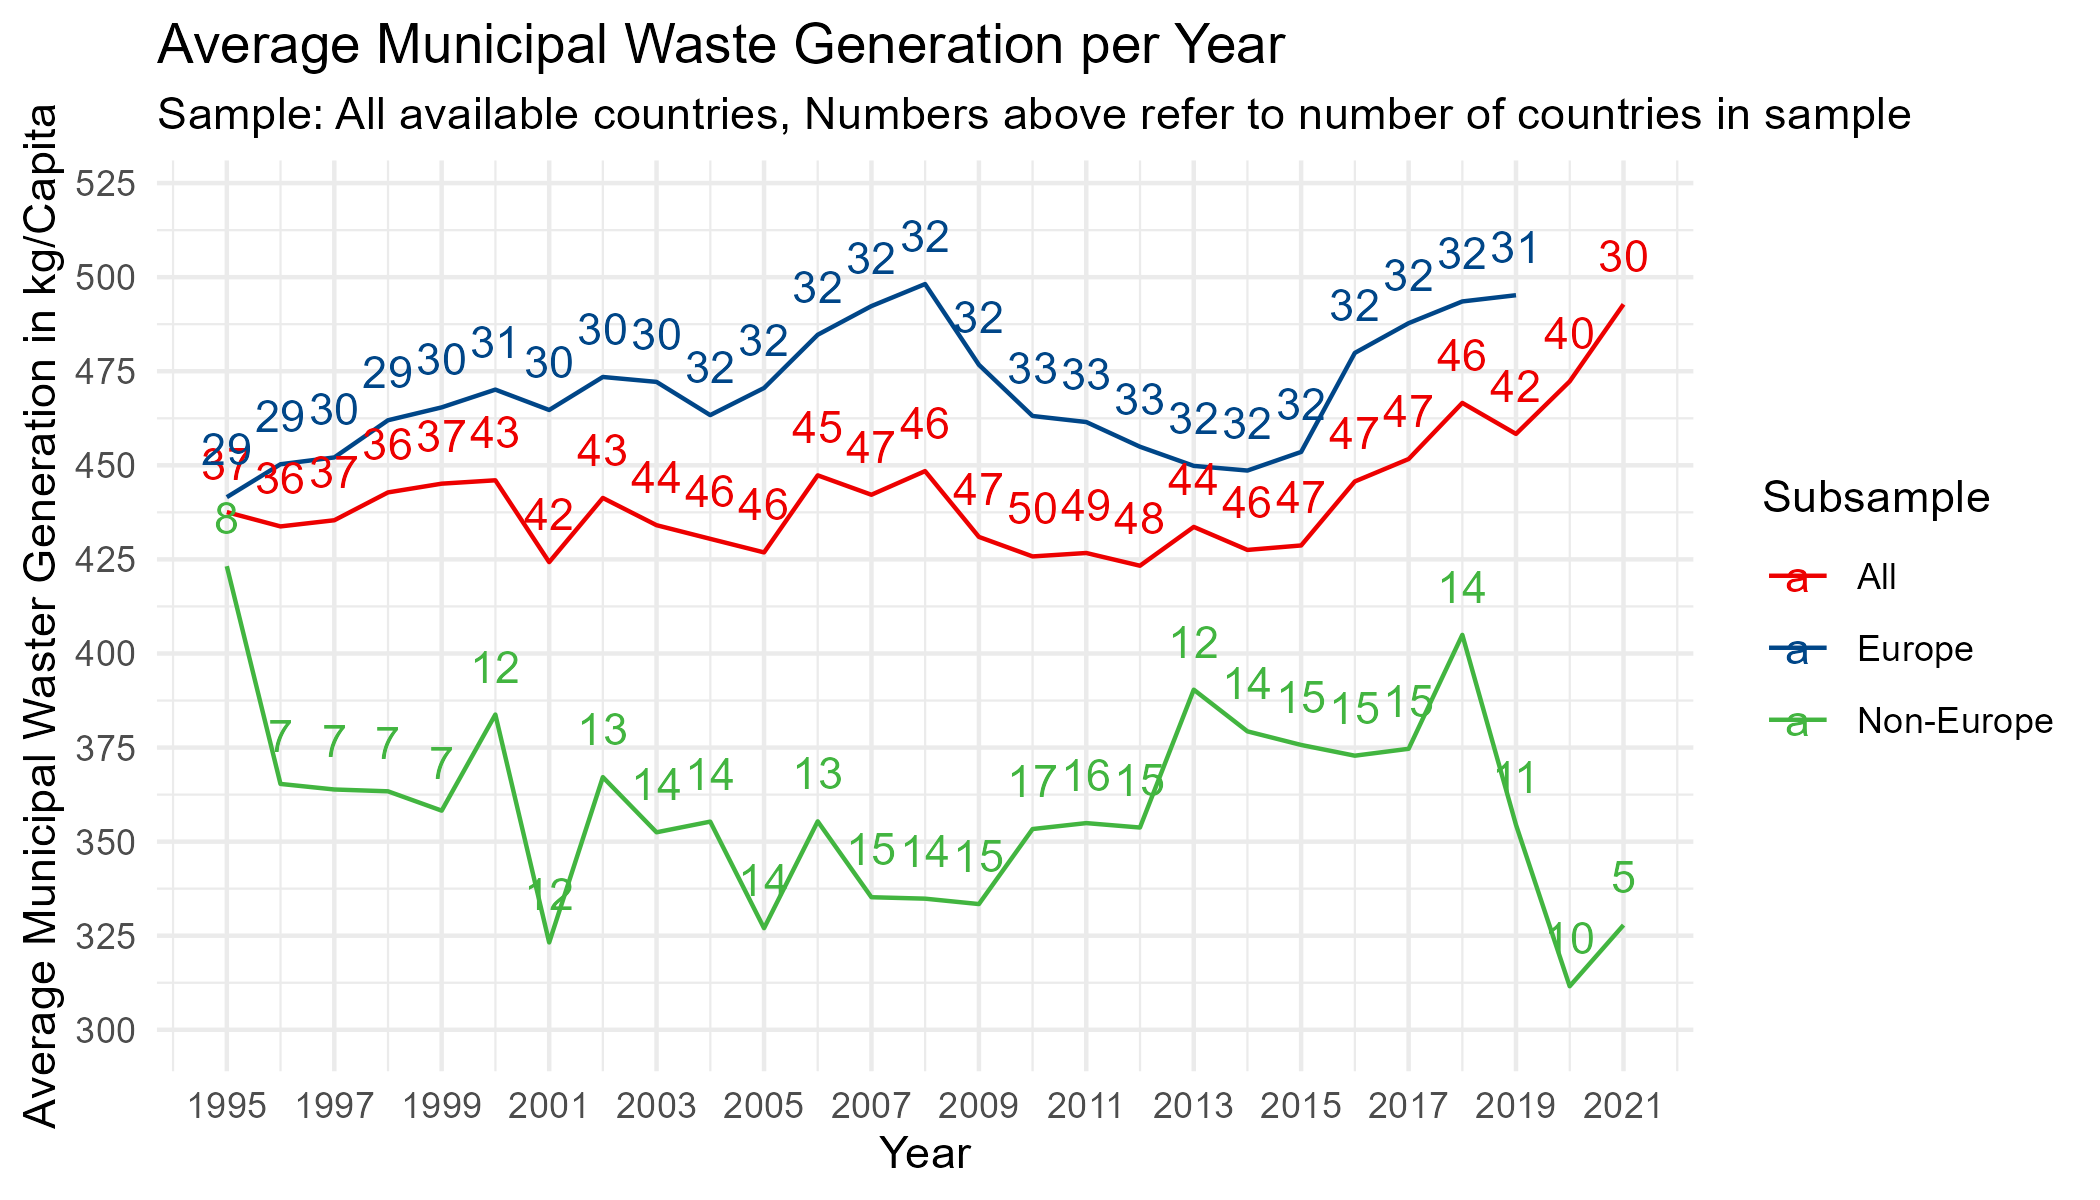
\includegraphics[scale=0.8]{../04_figures/AvgGen_pc.png}
\caption{Average Municipal Waste Generation in Kilogramms/Capita}
\label{fig:AvgWasteGen}
\end{figure}
In figure \ref{fig:AvgWasteGen}, a plot can be found showing the average municipal waste generation in kilograms per capita for different sub samples. The red line indicates the entire sample of countries, the blue line just looks at European countries and the green line covers all remaining countries. The numbers above the individual time points indicate the number of countries that have been used to compute the respective average. As can be seen from above, the high overall average is mainly driven by European countries as well as some special cases outside of Europe like the United States, New Zealand and Israel. 
\pagebreak
\section{Economic Analysis}


\pagebreak
\section{Conclusions}

\pagebreak
\section{Appendix}
\subsection{Histogram of Recycling Rates in 2015}

\begin{figure}[h]
\centering
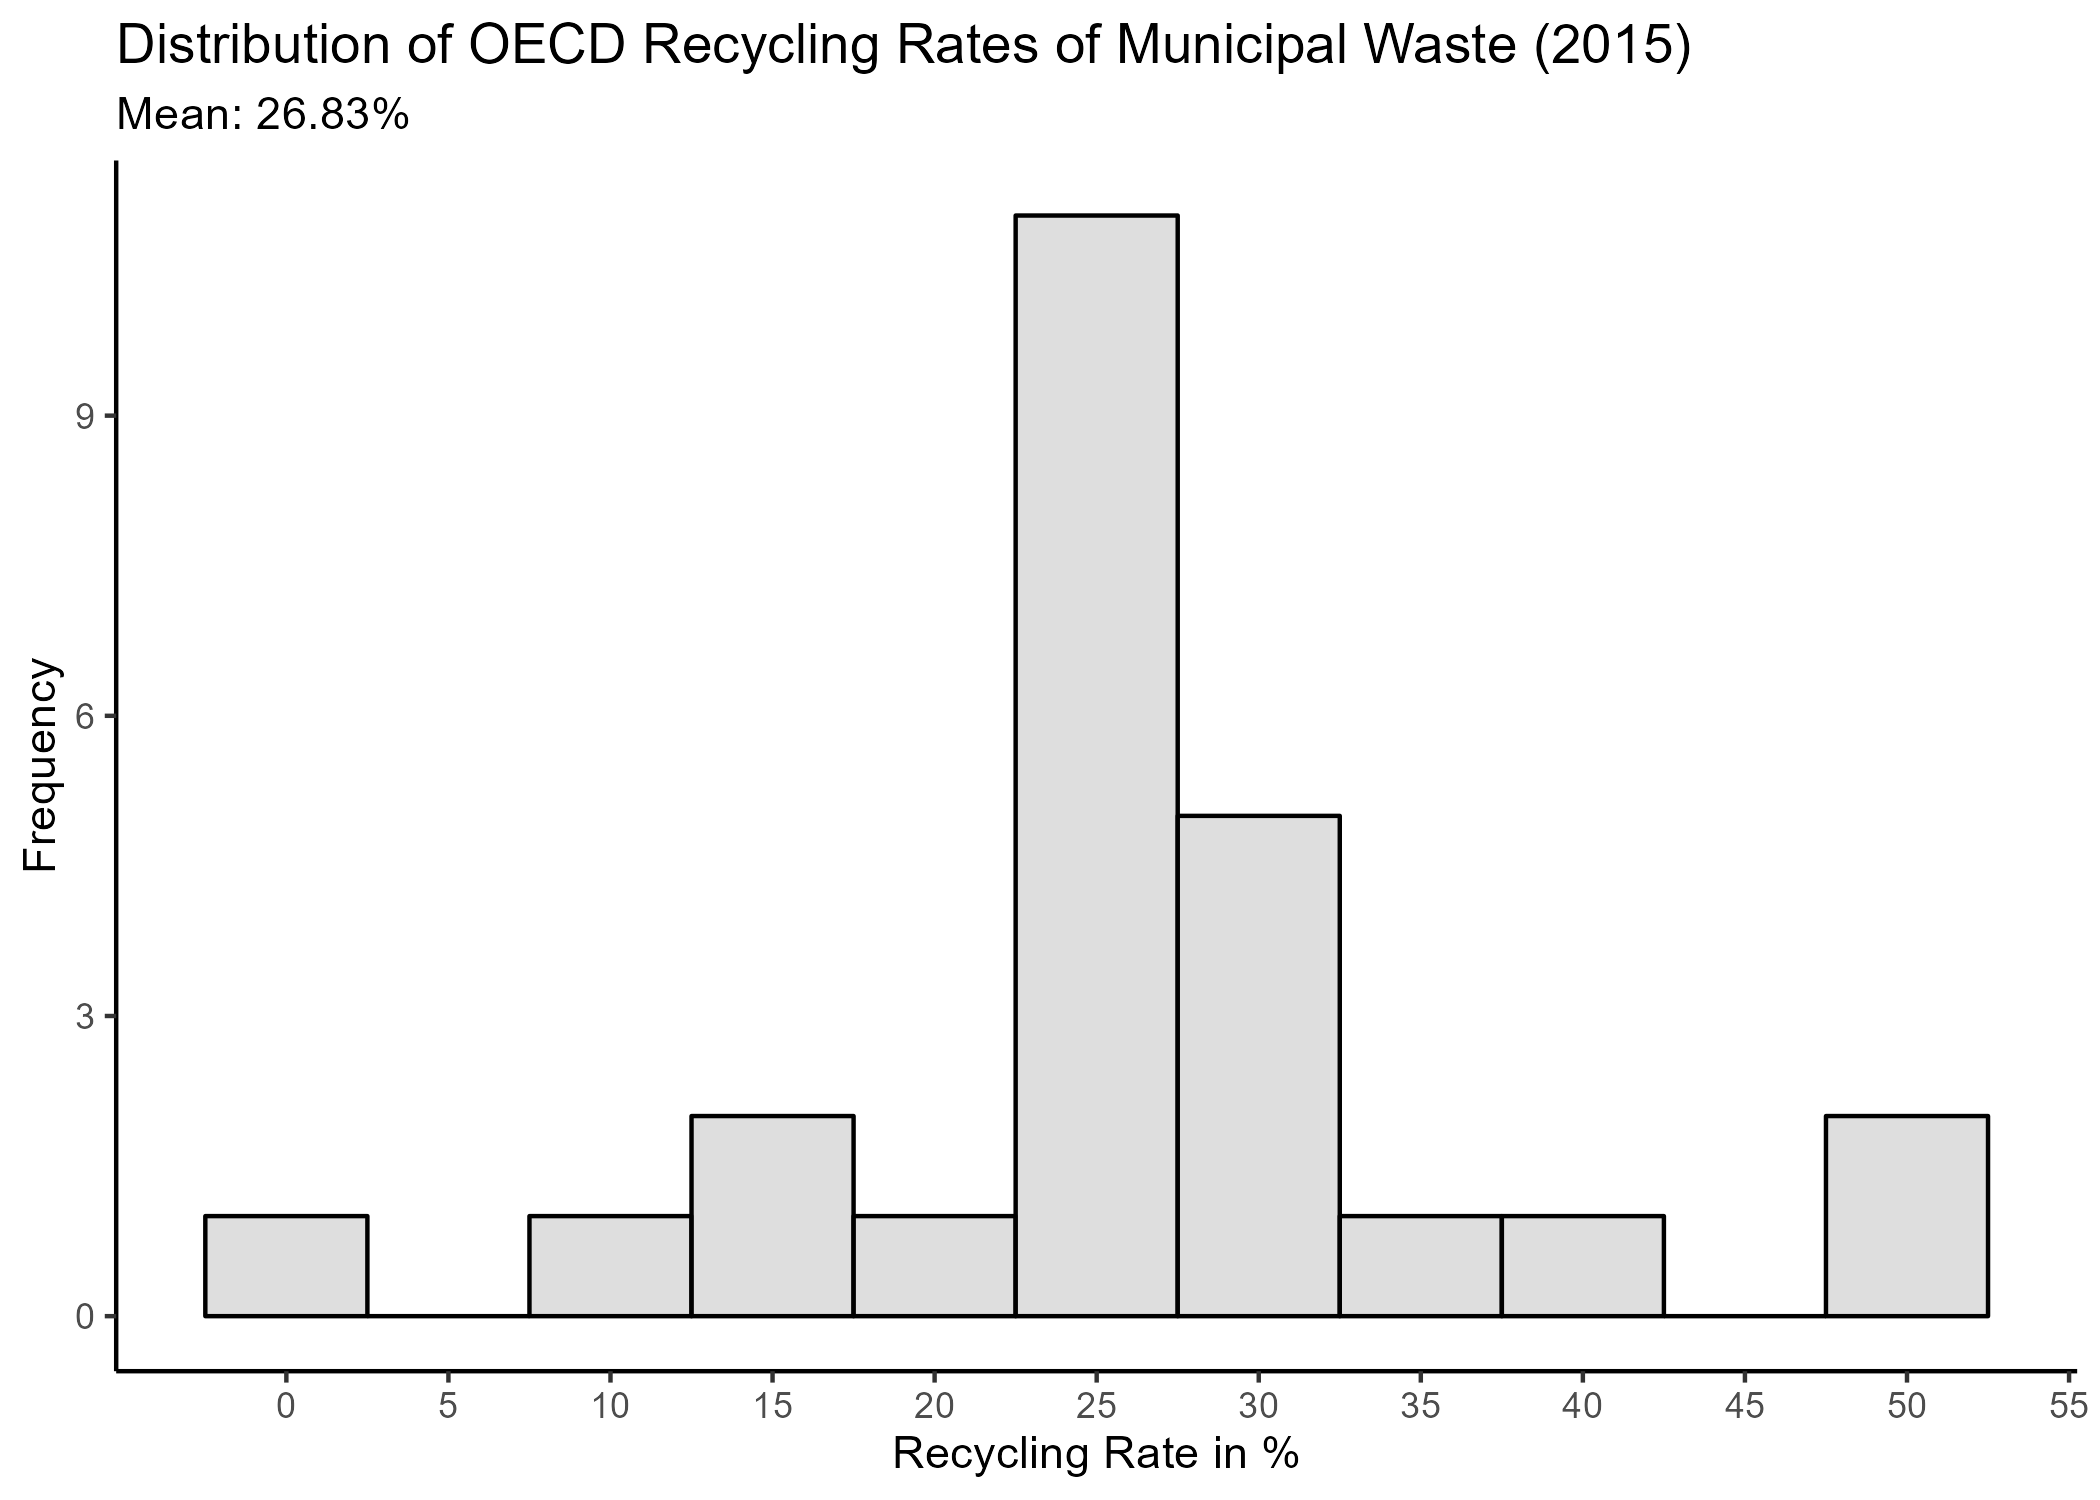
\includegraphics[scale=0.65]{../04_figures/hist_recyclingrates.png}
\caption{Histogram of Municipal Waste Recycling Rates of OECD Countries in 2015}
\label{fig:histrecycling}
\end{figure}

\subsection{Histogram of Average Year-on-Year Kilogram per Capita Growth Rates}

\begin{figure}[h]
\centering
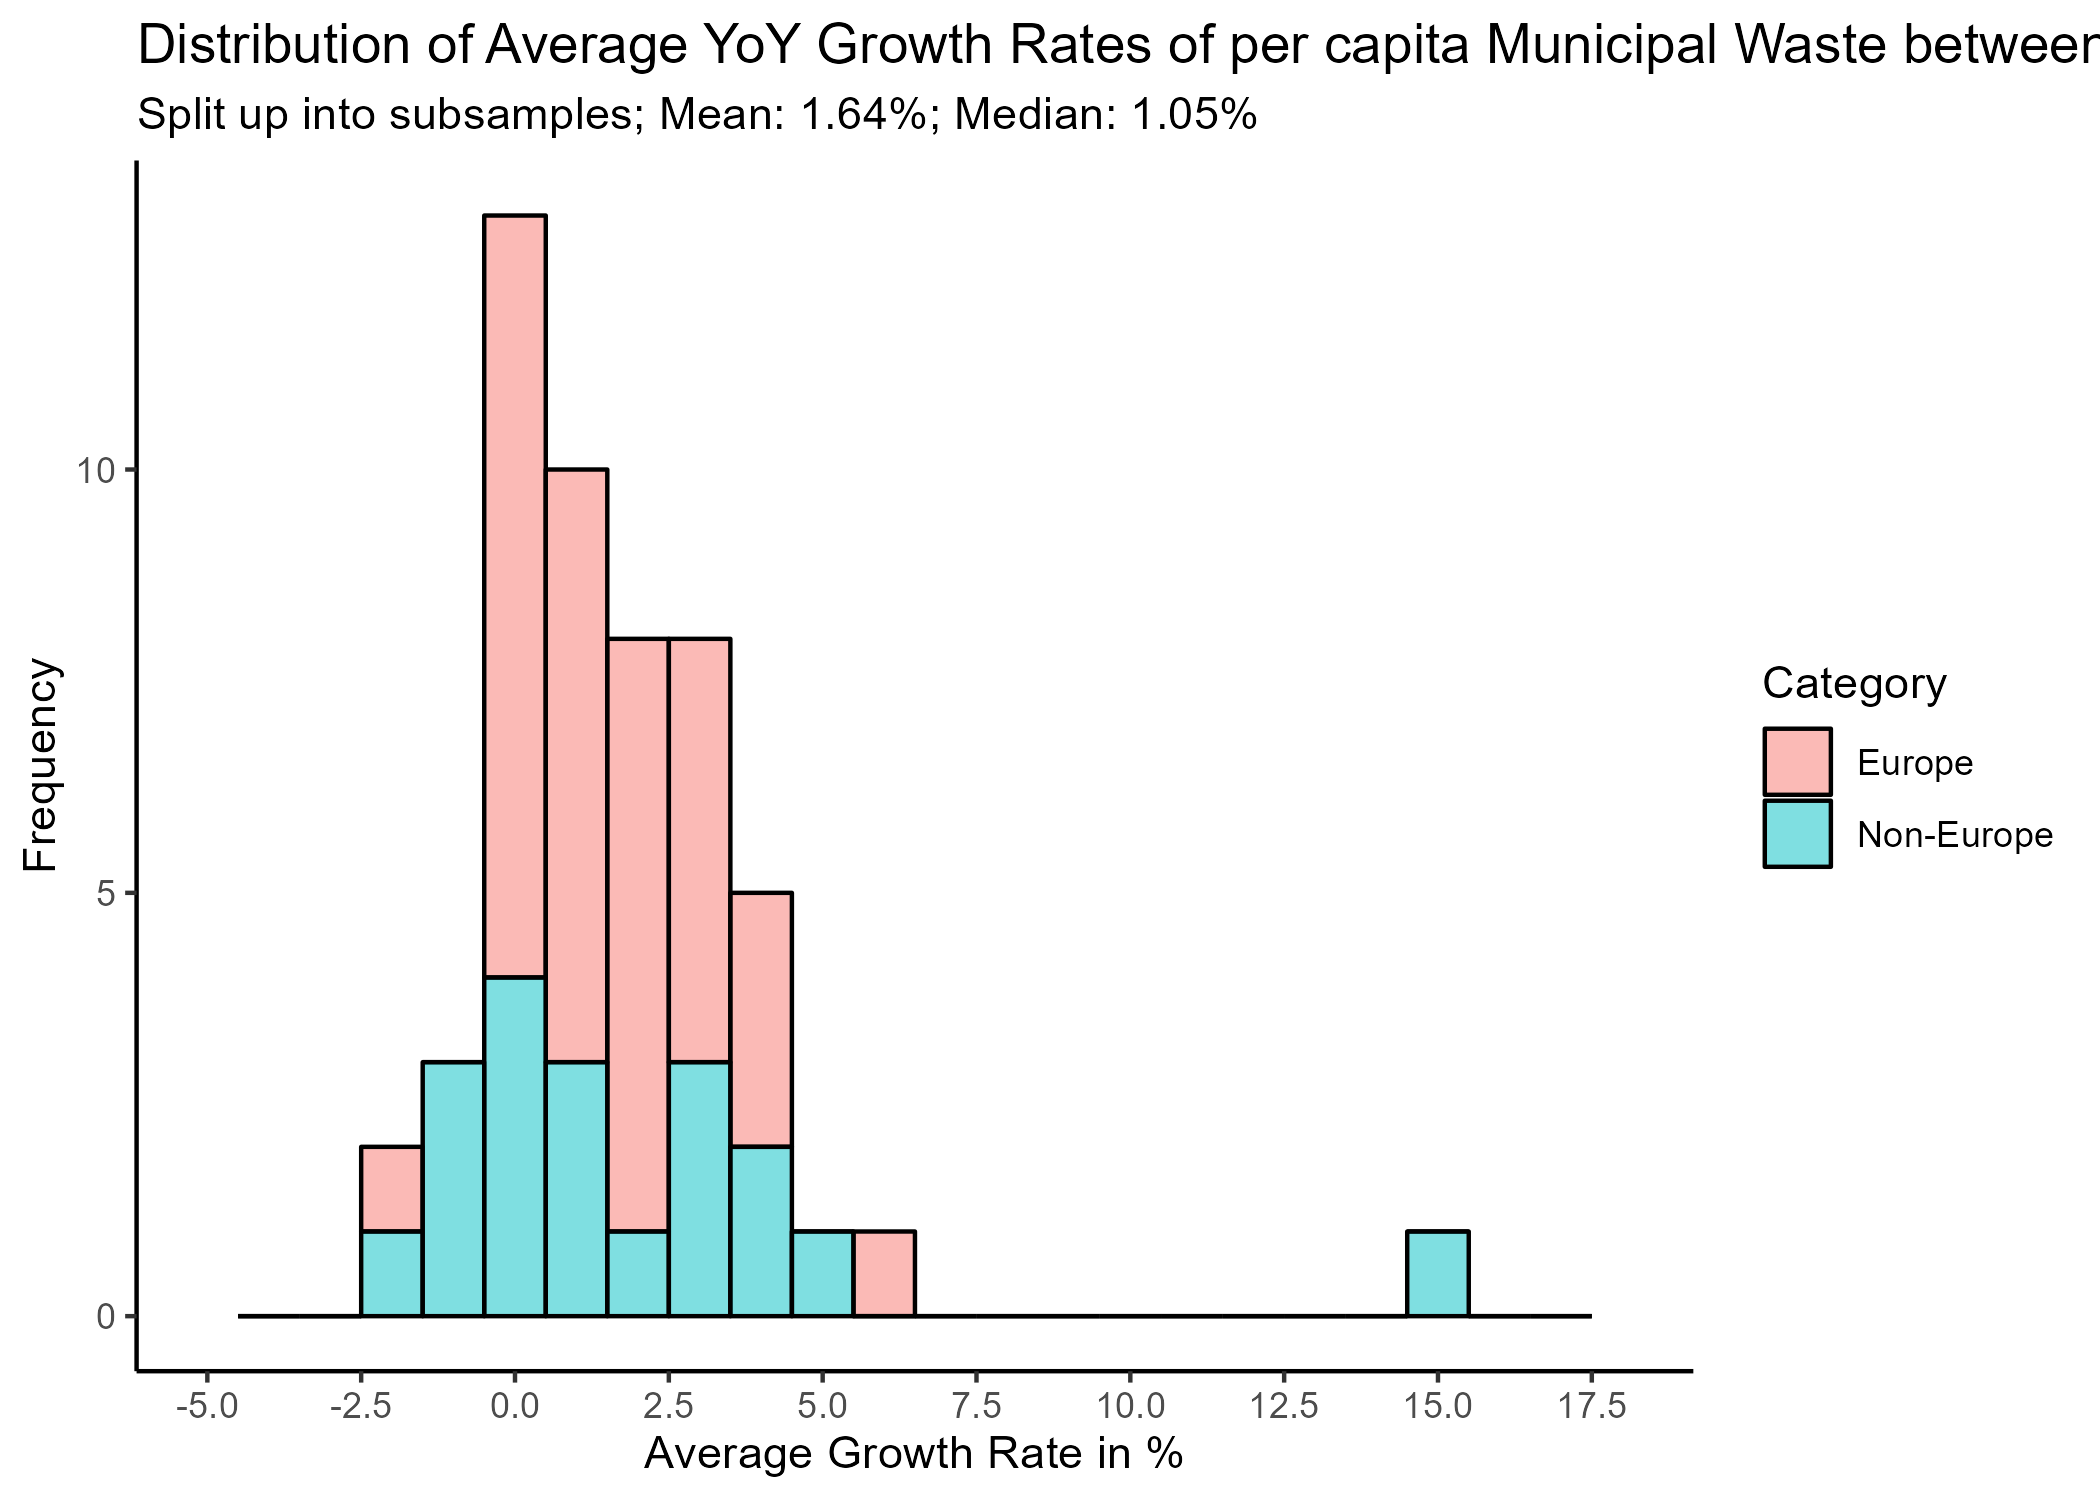
\includegraphics[scale=0.65]{../04_figures/hist_growthrates.png}
\caption{Histogram of Municipal Waste Recycling Rates of OECD Countries in 2015}
\label{fig:histgrowthrates}
\end{figure}


\pagebreak
\pagenumbering{roman}
\setcounter{page}{\thesavepage}
\pagestyle{plain}
\addcontentsline{toc}{section}{References}
%\bibliographystyle{apalike}
%\bibliography{ref.bib}
\printbibliography[]
\clearpage
\appendix
\end{document}
